\documentclass{ctexart}
\usepackage{amsmath,amssymb,bm}
\DeclareSymbolFont{EulerExtension}{U}{euex}{m}{n}
\DeclareMathSymbol{\euintop}{\mathop} {EulerExtension}{"52}
\DeclareMathSymbol{\euointop}{\mathop} {EulerExtension}{"48}
\let\intop\euintop
\let\ointop\euointop
\pagestyle{plain}
\begin{document}
\tableofcontents
\newpage

\section{\leftline{一个换元的常用方法}}

在曲线积分的计算中,经常会遇到两条曲面相交形成的曲线的积分.在这一类中,大部分都是圆柱(椭圆柱)和平面相交或球(椭球)和平面相交形成的圆或椭圆,那么如何写出这样的曲线的参数方程,进而求曲线积分呢?
\newline
\newline
\textbf{例:}求球面$x^{2}+y^{2}+z^{2}=a^{2}$与平面$x+y+z=0$相交形成的曲线的参数方程.

这种题都是一个二次式和一个一次式.首先需要在在二次式中通过一次式消去一个变元,这个题中我们消去$z$,变为$x^{2}+y^{2}+(-x-y)^{2}=a^{2}$,整理得
$$x^{2}+xy+y^{2}=\frac{a^{2}}{2}$$
然后把$x$看成未知量,$y$看成参数进行配方$x^{2}+xy+\frac{y^{2}}{4}+\frac{3y^{2}}{4}=\frac{a^{2}}{2}$,即
$$\left(x+\frac{y}{2}\right)^{2}+\left(\frac{\sqrt{3}y}{2}\right)^{2}=\frac{a^{2}}{2}$$
三角换元,有$x+\frac{y}{2}=\frac{a}{\sqrt{2}}\mathrm{cos}\ \theta,\frac{\sqrt{3}y}{2}=\frac{a}{\sqrt{2}}\mathrm{sin}\ \theta$
解出$x,y$后再利用一次式$x+y+z=0$求出$z$
\begin{align}
x&=a\left(\frac{1}{\sqrt{6}}\mathrm{cos}\ \theta+\frac{1}{\sqrt{2}}\mathrm{sin}\ \theta\right)\nonumber\\
y&=a\left(-\frac{2}{\sqrt{6}}\mathrm{cos}\ \theta\right)\nonumber\\
x&=a\left(\frac{1}{\sqrt{6}}\mathrm{cos}\ \theta-\frac{1}{\sqrt{2}}\mathrm{sin}\ \theta\right)\nonumber
\end{align}
\newline
\newline
求下列曲面的交线的参数方程

(1)$x^{2}+y^{2}=1,x+y+z=0$

(2)$x^{2}+y^{2}+z^{2}=a^{2},x=y$
\section{\leftline{第一型曲线(面)积分}}

第一型曲线积分的计算方法有参数换元和化为显式方程两种,而第一型曲面积分主要考显式方程,参数方程很少考察(所以一般的第一型曲面积分都要解出$z=f(x,y)$).
别忘了曲线积分化为定积分时要乘的式子.
(1)计算:$$\int_{\Gamma}xy\mathrm{d}s$$
其中$\Gamma$为球面$x^{2}+y^{2}+z^{2}=a^{2}$与平面$x+y+z=0$交成的圆周.

(2)计算:$$\int_{\Gamma}\sqrt{x^{2}+y^{2}}\mathrm{d}s$$
其中$\Gamma$为圆周$x^{2}+y^{2}=ax$.(容易算错)

(3)计算:$$\iint_{\Sigma}(xy+yz+zx)\mathrm{d}\sigma$$
其中$\Sigma$是$z=\sqrt{x^{2}+y^{2}}$被圆柱$x^{2}+y^{2}=2x$所截下的部分.(提示:利用对称性简化积分)

(4)求$$\iint_{S}\sqrt{x^{2}+y^{2}}\mathrm{d}S$$
$S$为锥面$z=\sqrt{x^{2}+y^{2}}$与平面$z=1$所围立体的表面.
\newline
\newline
注意,做题时要看清楚被积区域,如(4)中立体的表面是指侧面加上底面,而不是只有侧面.
\section{\leftline{第二型曲线(面)积分}}
第二型曲线积分需要注意积分的方向,通过给定的积分路径确定化为定积分的积分区间.如从(1,0)到(0,1)的直线$L$上的积分$\int_{L}f(x,y)\mathrm{d}x$,如果要消掉y转化为定积分,那么x应该从1积分到0,而不是0到1,积分变为$\int_{1}^{0}f(x,1-x)\mathrm{d}x$(不要默认定积分的上限总是比下限大,积分下限总是积分起点的横(纵)坐标值,积分上限总是终点的横(纵)坐标值)
\newline
\newline
(1)求$\int_{\Gamma}x\mathrm{d}y$,$\Gamma$是直线$2x+y=1$与两坐标轴组成的三角形,沿逆时针方向.
\newline
\newline
假如题目已经给出了参数方程,如果需要计算二重积分,则题目一般会说明曲线的正向是参数增加的方向,假如没有给出如何参数化,并且显化又不方便的就只能先化为参数方程然后自行判断参数怎样变化.对于二维的情况还算比较简单,基本上就是(广义)极坐标换元(不能用极坐标的基本上都能用显化来解决),逆时针就是$\theta$增加的方向,顺时针就是减少.

如果是在三维中,情况就不是这么简单了,对于下面这个题,由本文开头讲述的换元方法可以求出参数方程,但是如何确定参数增加对应的是曲线的正向,还是参数减少对应的是曲线的正向呢?
\newline
\newline
(2)求$$I=\int_{C}(y-z)\mathrm{d}x+(z-x)\mathrm{d}y+(x-y)\mathrm{d}z$$
其中$C$为球面$x^{2}+y^{2}+z^{2}=a^{2}$与平面$y=x\mathrm{tan}\ \alpha,(0<\alpha<\frac{\pi}{2})$交成的圆周,从$Ox$轴的正向看去,圆周沿逆时针方向.(如下图)

\begin{figure}[h!]

  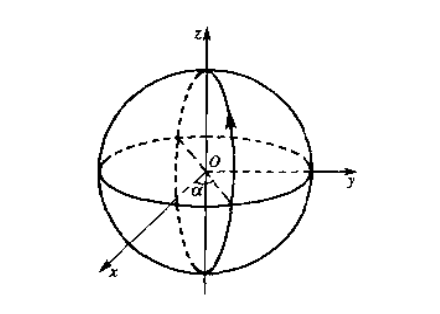
\includegraphics[width=6cm]{2.png}\\
\end{figure}

以上题为例,易求出参数方程$x=a\mathrm{cos}\ \alpha\mathrm{cos}\ t,y=a\mathrm{sin}\ \alpha\mathrm{cos}\ t,
z=a\mathrm{sin}\ t,$.这时,找一个比较简单的点,不妨这个点A为$(0,0,a)$,这时对应参数$t=\pi/2$,由图,在A点处,假如曲线朝着正向前进,那么A的x坐标会减少,那么对应到参数上$x=a\mathrm{cos}\ \alpha\mathrm{cos}\ t$当$t=\pi/2$时,假如t增大x坐标会减少,t减少x坐标会增大,所以正向的方向就是参数增加的方向.(同理,用y坐标也可以判断出来.\textbf{注意:}对于这个题来讲用z坐标是不能判断的.因为当t为$\pi/2$时,无论t增大还是减少,z坐标都会减少,除非在曲线上换一个点A,比如取A是曲线和xoy平面的交点)
\newline
\newline
对于曲面积分,参数换元基本上不会考,一般是考显化,并且都是显化$z$,变成$z=f(x,y)$的形式,然后把$P,Q,R$中的$z$全部换成$f(x,y)$,
\begin{align}
\ \ &\iint_{\Sigma}P(x,y,z)\mathrm{d}y\mathrm{d}z+Q(x,y,z)\mathrm{d}z\mathrm{d}x+R(x,y,z)\mathrm{d}x\mathrm{d}y\nonumber\\
=&\pm\iint_{D}-P(x,y,f(x,y))\frac{\partial z}{\partial x}-Q(x,y,f(x,y))\frac{\partial z}{\partial y}+R(x,y,f(x,y))\mathrm{d}x\mathrm{d}y\nonumber
\end{align}
这个公式不用死记硬背

1)因为是把这个曲线积分的积分区域投影到xoy平面上,首先要把空间区域$\Sigma$在xoy上的投影$D$求出来,然后要看曲面的正法向量和z轴的夹角,若是锐角则前面是正号,若是钝角则前面加负号,所谓的正法向量是指指向曲面所给方向的向量.比如:题目规定曲面是半球$x^{2}+y^{2}+z^{2}=a^{2},z>0$的外侧,那么对于任意球上一点(x,y,z),这一点的法向量有两个,一个是指向球心的向量,另外一个是由球心指向(x,y,z)的向量,由于曲面是球的外侧,那么它对应的正法向量也应该指向球的外侧,即由球心指向(x,y,z)的向量,又因为当$z>0$ 时这个向量和z 正半轴夹角为锐角(判断锐角还是钝角不用算,想象一下图形就立刻出来了),所以换元后前面是正号.假如规定的是上半球的内侧,那么对应的正法向量就是指向半球内侧的那个法向量,这个法向量和z 轴正向的夹角为钝角,所以换元后需要在前面加负号,假如给的是整个的球$x^{2}+y^{2}+z^{2}=a^{2}$,这时无论是外侧还是内侧对应的正法向量和z 轴的夹角都不是恒为锐角或钝角,那这时换元公式前面的$\pm$怎么确定呢?这时只能把球面分成上半球面和下半球面了,然后分别判断计算再相加(不过对于这种闭合曲面的曲面积分都用高斯定理更简单)

2)对于换元中把$P\mathrm{d}y\mathrm{d}z$换成$-P\frac{\partial z}{\partial x}\mathrm{d}x\mathrm{d}y$也不需要死记硬背,因为我们做的是$z=f(x,y)$变化,所以首先要把$P$中所有的$z$换成$f(x,y)$,而对于dydz,因为z是x的函数(这时将y看成常数),所以有$\mathrm{d}y\mathrm{d}z=\frac{\partial z}{\partial x}\mathrm{d}y\mathrm{d}x$,而dydx=-dxdy(原理是向量叉乘换序后互为相反数)所以$\mathrm{d}y\mathrm{d}z=-\frac{\partial z}{\partial x}\mathrm{d}x\mathrm{d}y$
同理可推出$Q\mathrm{d}z\mathrm{d}x$和$R\mathrm{d}x\mathrm{d}y$
\newline
\newline
(3)计算第二型曲面积分$$\iint_{\Sigma}x^{4}\mathrm{d}y\mathrm{d}z+y^{4}\mathrm{d}z\mathrm{d}x+z^{4}\mathrm{d}x\mathrm{d}y$$
$\Sigma$是$x^{2}+y^{2}+z^{2}=a^{2}$的内侧.
\newline
\newline
(4)计算第二型曲面积分$$\iint_{\Sigma}z\mathrm{d}x\mathrm{d}y$$
$\Sigma$是$\frac{x^{2}}{a^{2}}+\frac{y^{2}}{b^{2}}+\frac{z^{2}}{c^{2}}=1$的外侧.
\section{\leftline{第一型,第二型曲线积分的转化,green公式}}
对于曲线积分,有$$\int_{\Gamma}P\mathrm{d}x+Q\mathrm{d}y+R\mathrm{d}z=\int_{\Gamma}(P\mathrm{cos}\ \alpha+Q\mathrm{cos}\ \beta+R\mathrm{cos}\ \gamma)\mathrm{d}s$$

注意$\alpha,\beta,\gamma$是\textbf{沿曲线正方向的切向量}在每一点与x,y,z轴正半轴的夹角,是关于x,y,z的函数而不是常数.(并且有$\mathrm{cos}^{2}\ \alpha+\mathrm{cos}^{2}\ \beta+\mathrm{cos}^{2}\ \gamma=1$),合理使用两个积分的转化会使得某些题(大部分是证明题)变得简单.
\newline
\newline
\newline
(1)设$M=\mathrm{max}(\sqrt{P^{2}(x,y,z)+Q^{2}(x,y,z)+R^{2}(x,y,z)})$,$c$为被积曲线$\Gamma$的长度,证明:$$\left|\int_{\Gamma}P\mathrm{d}x+Q\mathrm{d}y+R\mathrm{d}z\right|\leq Mc$$
\newline
提示:
\begin{align}
P\mathrm{d}x+Q\mathrm{d}y+R\mathrm{d}z&=(P\mathrm{cos}\ \alpha+Q\mathrm{cos}\ \beta+R\mathrm{cos}\ \gamma)\mathrm{d}s\nonumber\\
&\leq (\sqrt{P^{2}+Q^{2}+R^{2}}\sqrt{\mathrm{cos}^{2}\ \alpha+\mathrm{cos}^{2}\ \beta+\mathrm{cos}^{2}\ \gamma})\mathrm{d}s\nonumber\\
&=\sqrt{P^{2}+Q^{2}+R^{2}}\mathrm{d}s\nonumber\\
&\leq M\mathrm{d}s\nonumber
\end{align}
其中用到了Cauchy不等式$(a_{1}b_{1}+a_{2}b_{2}+a_{3}b_{3})^{2}\leq (a_{1}^{2}+a_{2}^{2}+a^{2}_{3})(b_{1}^{2}+b_{2}^{2}+b^{2}_{3})$
\newline
\newline
对于Green公式,大部分的\textbf{闭曲线}(比如圆,椭圆)都可以用green来简化计算,而对于\textbf{不规则的路径,或者过于复杂的被积函数},一般都需要用green来求解,对于\textbf{没有给出具体的积分路径}的题,只能用green求解,另外green的变形还能用于计算某些图形的面积$\iint_{D}\mathrm{d}x\mathrm{d}y=\frac{1}{2}\int_{\partial D}x\mathrm{d}y-y\mathrm{d}x$.
\newline
\newline
(2)用曲线积分求星形线$x=a\mathrm{cos}^{3}t,x=a\mathrm{sin}^{3}t$,所围图形的面积,其中$a>0$为常数.
\newline
\newline
(3)求$$I=\int_{C}\sqrt{x^{2}+y^{2}}\mathrm{d}x+y(xy+\mathrm{ln}(xy+\sqrt{x^{2}+y^{2}}))\mathrm{d}y$$,其中$C$是以点A(1,1),B(2,2),E(3,1)为顶点的三角形的正向边界线(被积函数过于复杂,需要green).

(\textbf{牢记:}所谓的一个曲面的正向边界线是指:对于一个曲面$D$,一个人沿着$D$的边界$\partial D$行进,区域$D$总是在这个人的左手边,这样前进的方向就是$D$的正向,否则相反的方向是正向)
\newline
\newline
(4)求$$I=\int_{C}(\mathrm{e}^{x}\mathrm{sin}\ y-m(x+y))\mathrm{d}x+(\mathrm{e}^{x}\mathrm{cos}\ y-m)\mathrm{d}y$$,其中$C$是上半圆周$x^{2}+y^{2}=ax$,沿$x$增加的方向.(添加适当的辅助线使积分区域成为闭合曲线用green算出积分值后再减去添加的辅助线上的积分)
\newline
\newline
(5)求$$\int_{L}\frac{(x+y)\mathrm{d}x-(x-y)\mathrm{d}y}{x^{2}+y^{2}}$$其中$L$是位于上半平面从点(-1,0)到(1,0)的任意光滑线段.(积分路径不确定,必须用green)
\newline
\newline
(6)单变量函数$f$连续可微,$C$是任意一条分段光滑的封闭曲线,证明:$$\int_{C}f(xy)(y\mathrm{d}x+x\mathrm{d}y)=0$$和$$\int_{C}f(x^{2}+y^{2})(y\mathrm{d}x+x\mathrm{d}y)=0$$
\newline
\newline
假如对于一个区域$D$中某些点处green不适用,那么可以选择挖去这点的邻域$E$,然后用green计算剩余部分$D$的正向加$E$的负向的积分,即区域$D\setminus E$的二重积分,用其他方法计算$E$的正向的曲线积分.
\newline
\newline
(7)计算积分$$I=\int_{\Gamma}\frac{x\mathrm{d}y-y\mathrm{d}x}{x^{2}+y^{2}}$$其中$\Gamma$是任意一条包含原点但不通过原点的光滑封闭曲线.(提示:挖掉半径足够小的圆$x^{2}+y^{2}\leq \varepsilon^{2}$)
\newline
\newline
\newline
可以与复变函数中的复积分进行类比来记忆曲线积分的一些结论(虽然我知道你一定不知道,但我还是想要把它写出来)

\textcircled{\footnotesize{1}} 一个二元函数$f(x,y)=P(x,y)+\mathrm{i}Q(x,y)$有连续的偏导数并且有$\frac{\partial P}{\partial y}=\frac{\partial Q}{\partial x}$ 就类似于复函数是解析函数(也叫全纯函数)

\textcircled{\footnotesize{2}} 满足$\frac{\partial P}{\partial y}=\frac{\partial Q}{\partial x}$,并且偏导数连续,则$P\mathrm{d}x+Q\mathrm{d}y$绕闭合曲线的积分为0,类似于Cauchy积分定理:解析函数沿闭曲线的积分为0

\textcircled{\footnotesize{3}} 当某点的$\frac{\partial P}{\partial y}$或$\frac{\partial Q}{\partial x}$不连续时,就不能用green,类似的,如果复函数在某个积分区域$D$的某些点不解析(这样的点叫做奇点),那么沿$\partial D$的积分也不一定为0.

\textcircled{\footnotesize{4}} 如上面的(10),在偏导数不连续的点(0,0),可以通过挖掉一个半径足够小的圆,使得圆内除了那个(0,0)外没有任何其他的偏导数不连续的点,这样的点在复变函数中对应着孤立奇点.继续观察(10)中(0,0)的点,发现无论圆的半径$\varepsilon$如何变化,积分都为$2\pi$,甚至积分曲线可以不是圆,只要是包含(0,0),并且曲线内除了(0,0) 没有其他的偏导数不连续的点,只要满足这两条,沿这条曲线的积分都为$2\pi$,这个恒定量$2\pi$在复变函数中对应着$z_{0}$处的留数,即$\frac{1}{2\pi\mathrm{i}}\int_{C}f(z)\mathrm{d}z$,其中闭合曲线$C$满足$f(z)$在且仅在$z_{0}$处不解析

\section{\leftline{第一,二型曲面积分的转化,Gauss,Stokes公式}}
对于曲面积分,有$$\int_{\Sigma}P\mathrm{d}y\mathrm{d}z+Q\mathrm{d}z\mathrm{d}x+R\mathrm{d}x\mathrm{d}y=\int_{\Gamma}(P\mathrm{cos}\ \alpha+Q\mathrm{cos}\ \beta+R\mathrm{cos}\ \gamma)\mathrm{d}\sigma$$

注意$\alpha,\beta,\gamma$是\textbf{曲线的正法向量}在每一点与x,y,z轴正半轴的夹角,是关于x,y,z的函数而不是常数.(并且有$\mathrm{cos}^{2}\ \alpha+\mathrm{cos}^{2}\ \beta+\mathrm{cos}^{2}\ \gamma=1$),合理使用两个积分的转化会使得某些题(大部分是计算题)变得简单.
\newline
\newline
\textbf{例:}\ \
曲面$\Sigma$是中心在原点,半径为$a$的球面,正向是外法线方向,计算积分$$I=\iint_{\Sigma}x\mathrm{d}y\mathrm{d}z+y\mathrm{d}z\mathrm{d}x+z\mathrm{d}x\mathrm{d}y$$

因为对于球来说,原点到该点的连线与该点的法向量共线,所以对于任意球上的一点$(x,y,z)$,该点的法向量就是$(kx,ky,kz)$,因为曲线的正向是外法线方向,所以$k>0$,再将这个向量单位化(因为$\mathrm{cos}^{2}\ \alpha+\mathrm{cos}^{2}\ \beta+\mathrm{cos}^{2}\ \gamma=1$),得到单位正法向量$\bm{n}=(x/a,y/a,z/a)$,即$(\mathrm{cos}\ \alpha,\mathrm{cos}\ \beta,\mathrm{cos}\ \gamma)=(x/a,y/a,z/a)$,带入到式子中有
\begin{align}
\iint_{\Sigma}x\mathrm{d}y\mathrm{d}z+y\mathrm{d}z\mathrm{d}x+z\mathrm{d}x\mathrm{d}y&=\iint_{\Sigma}\frac{x^{2}+y^{2}+z^{2}}{a}\mathrm{d}\sigma\nonumber\\
&=a\iint_{\Sigma}\mathrm{d}\sigma\nonumber\\
&=a\sigma (\Sigma)\nonumber\\
&=4\pi a^{3}\nonumber
\end{align}
其中$\sigma (\Sigma)$表示闭合曲面$\Sigma$的表面积.
\newline
\newline
\textbf{练一练!}

(1)$\Sigma$是三角形$\{(x,y,z):x,y,z\leq0,x+y+z=1\}$,法向量与$(1,1,1)$同向,计算积分
$$\iint_{\Sigma}x\mathrm{d}y\mathrm{d}z+y\mathrm{d}z\mathrm{d}x+z\mathrm{d}x\mathrm{d}y$$
(提示:单位正法向量$\bm{n}=(1,1,1)/\sqrt{3}$)

(2)设有流速场$\bm{F}=(yz,zx,xy)$,曲面$\Sigma$是圆柱体$x^{2}+y^{2}\leq a^{2},0\leq z\leq h$的表面,求流速场流出$\Sigma$的流量.(提示:$\Sigma$由三块曲面拼接而成,对于其中的圆柱面,其单位正法向量$\bm{n}=(x/a,y/a,0)$)
\newline
\newline
\newline
对于封闭曲面的曲面积分,首选gauss,不封闭的也可以通过增补使之成为封闭曲面然后减去增补的部分的曲面积分.(增补部分一般是一个平面,通常是一个半(椭)球,补上z=0平面,用gauss计算出积分再减去z=0平面的曲面积分.并且z=0的曲面积分很好计算,因为被积区域就是一个(椭)圆,并且可以将被积函数中的z全部换为0,并且由于平面的法向量和x轴,y 轴都垂直,所以dydz和dzdx为0,只需要计算dxdy的曲面积分)
\newline
\newline
注意区别被积曲面,是所有的表面都要参与积分,还是只需要积分曲面,不需要积分平面?一般而言,需要积分所有的面的都会描述为:曲面1,曲面2,曲面3\textbf{所围的立体的表面}的外(内)侧,只需要积分曲面的都会描述为:曲面4的外(内)侧或者曲面5被曲面6所截的部分的上(下)侧
\newline
\newline
(3)$S$是曲面$x^{2}+y^{2}=1,z=0,z=3$所围立体的全表面的外侧.计算$$\iint_{S}(x-y)\mathrm{d}x\mathrm{d}y+(y-z)x\mathrm{d}y\mathrm{d}z$$
(注意:用gauss时一定要看清楚后面的微元再求导,微元是dydz的只能对x求导,微元是dzdx的只能对y求导,微元是dxdy的只能对z求导.不要默认写在第一个的就要对x求导)
\newline
\newline
(4)$S$是上半球面$x^{2}+y^{2}+z^{2}=R^{2},z\leq 0$,取内侧,计算$$\iint_{S}x^{2}\mathrm{d}y\mathrm{d}z+y^{2}\mathrm{d}z\mathrm{d}x+z^{2}\mathrm{d}x\mathrm{d}y$$
\newline
\newline
如果我们将偏微分$\frac{\partial P}{\partial x}$看成偏微分算子$\frac{\partial }{\partial x}$和函数$P$的乘积的话,那么stokes有简便的记忆方法
$$\int_{\partial \Sigma}P\mathrm{d}x+Q\mathrm{d}y+R\mathrm{d}z=\iint_{\Sigma}\left|
\begin{array}{ccc}
\mathrm{d}y\mathrm{d}z&\mathrm{d}z\mathrm{d}x&\mathrm{d}x\mathrm{d}y\\
\frac{\partial }{\partial x}&\frac{\partial }{\partial y}&\frac{\partial }{\partial z}\\
P&Q&R
\end{array}
\right|$$
然后将第一行展开即为所求.

stokes不是考试的重点,练几个简单的题就可以了.(大部分的三维曲线积分都能利用参数化来计算出,所以stokes用处不大)

对于stokes公式来说,如何将曲线的方向转化为曲面的方向是非常重要的,这需要用右手螺旋定则:\textbf{用右手握住有向闭合曲线,让四指指向曲线的正向,那么拇指指向就是曲面正法向量的方向.}题目中经常给的条件是从某个点看去,曲线是逆(顺)时针绕行的.通过右手螺旋定则,可以得到结论:\textbf{若从某点看上去,曲线是逆时针方向绕行的,那么该曲面的正法向量方向就应该指向那个点,反之,就应该远离那个点.}

比如,某个题目中给出条件:$\Gamma$是平面$x+y=2$和球面$x^{2}+y^{2}+z^{2}=2{x+y}$交成的圆周,从原点看去,顺时针方向是$\Gamma$的正向.那么如果取$\Gamma$围成的曲面是平面$x+y=2$的一部分,(法向量可能是$\pm(1/\sqrt{2},1\sqrt{2},0)$)由上面的结论,远离原点的方向就是正法向量方向,又因为$x,y$都大于0(想想为什么),所以远离原点的方向就是$(1/\sqrt{2},1\sqrt{2},0)$,即正单位法向量.有了正法向量后既可以将第二型积分化为第一型,也可以化为二重积分.

假如已经求得了曲面积分,想把它转化为二重积分(不妨设将其投影到xoy平面上),需要计算所给曲线在xoy平面上的投影$\Gamma$,然后计算被积区域是$\Gamma$的内部的二重积分.对于所有的题来说,一条空间曲线由两个曲面的交线给出(假如一条曲线是以参数方程的形式给出的,那就不需要用stokes了),联立两个曲面的方程,消去z,就得到了在xoy上的投影.

比如,某个题目中给出条件:$\Gamma$为圆周$x^{2}+y^{2}+z^{2}=a^{2},x+y+z=0$,那么这条曲线在xoy的投影就是$x^{2}+y^{2}+(x+y)^{2}=a^{2}$.
\newline
\newline
\textbf{例:}
计算曲线积分$$I=\int_{\Gamma}(y^{2}+z^{2})\mathrm{d}x+(z^{2}+x^{2})\mathrm{d}y+(x^{2}+y^{2})\mathrm{d}z$$
其中$\Gamma$为$x^{2}+y^{2}+z^{2}=2ax,x^{2}+y^{2}=2bx,(z\leq 0,0<b<a)$.从z轴的正向看去,$\Gamma$是逆时针方向绕行的.
\begin{figure}[h!]
  \centering

  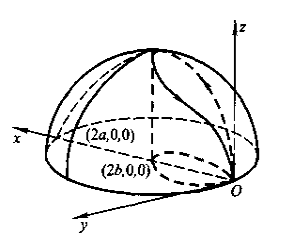
\includegraphics[width=6cm]{3.png}\\

\end{figure}

由于在z轴正向是逆时针,所以球面上的正法向量应该指向z轴正向,即$\mathrm{cos}\ \alpha=\frac{x-a}{a},\mathrm{cos}\ \beta=\frac{y}{a},\mathrm{cos}\ \gamma=\frac{z}{a},$
用$\Sigma$记曲线$\Gamma$在球面$x^{2}+y^{2}+z^{2}=2ax$上围出的那块曲面,
用stokes转化为第二型曲面积分$$2\iint_{\Sigma}(y-z)\mathrm{d}y\mathrm{d}z+(z-x)\mathrm{d}z\mathrm{d}x+(x-y)\mathrm{d}x\mathrm{d}y$$
再根据正单位法向量转化为第一型曲面积分,$$2\iint_{\Sigma}(z-y)\mathrm{d}\sigma$$

由于$\Sigma$关于xoz平面对称,所以$\iint_{\Sigma}y\mathrm{d}\sigma=0$,而$\Sigma$在xoy上的投影应该为两个曲面消掉z的方程表示出,但因为有一个曲面$x^{2}+y^{2}=2bx$ 本身不含z,所以投影区域$D$就是圆盘$x^{2}+y^{2}=2bx$.所以
\begin{align}
2\iint_{\Sigma}(z-y)\mathrm{d}\sigma&=2\iint_{\Sigma}z\mathrm{d}\sigma\nonumber\\
&=2\iint_{D}z\cdot \frac{a}{z}\mathrm{d}x\mathrm{d}y\nonumber\\
&=2\pi ab^{2}\nonumber
\end{align}
\newline
\newline
一般而言,三维的曲面积分最好是用参数换元,stokes容易算错,只有参数换元不方便时才要考虑stokes
\section{\leftline{梯度,散度,旋度,保守场,势函数}}
这部分内容比较简单,一般都会出判断是否为保守场并求势函数的问题.

记住各种量的计算方法

设数量场$f(x,y,z)$,向量场$\bm{F}(x,y,z)=(P(x,y,z),Q(x,y,z),R(x,y,z))$

\begin{align}
\mathrm{grad}f&=\nabla f=\left(\frac{\partial f}{\partial x},\frac{\partial f}{\partial y},\frac{\partial f}{\partial z}\right)\nonumber\\
\mathrm{div}\bm{F}&=\frac {\partial P}{\partial x}+\frac {\partial Q}{\partial y}+\frac {\partial R}{\partial z}\nonumber\\
\mathrm{rot}\bm{F}&=\left(\frac{\partial R}{\partial y}-\frac{\partial Q}{\partial z},\frac{\partial P}{\partial z}-\frac{\partial R}{\partial x},\frac{\partial Q}{\partial x}-\frac{\partial P}{\partial y}\right)\nonumber\\
&=\left(\frac{\partial R}{\partial y}-\frac{\partial Q}{\partial z}\right)\bm{i}+\left(\frac{\partial P}{\partial z}-\frac{\partial R}{\partial x}\right)\bm{j}+\left(\frac{\partial Q}{\partial x}-\frac{\partial P}{\partial y}\right)\bm{k}\nonumber\\
&=\left|
\begin{array}{ccc}
\bm{i}&\bm{j}&\bm{k}\\
\frac{\partial }{\partial x}&\frac{\partial }{\partial y}&\frac{\partial }{\partial z}\\
P&Q&R
\end{array}
\right|\nonumber
\end{align}

记忆旋度公式时采用行列式较为简单.

一般的题都是先证明是无旋场,然后再求势函数,求势函数的时候一般是采取从$(0,0,0)$到$(x_{0},y_{0},z_{0})$的积分(若$(0,0,0)$无定义,则换一个其他的方便计算的点如$(a,0,0)$), 即
$$\int_{(0,0,0)}^{(x,y,z)}P\mathrm{d}x+Q\mathrm{d}y+R\mathrm{d}z$$,一般采用$(0,0,0)$到$(x_{0},0,0)$到$(x_{0},y_{0},0)$到$(x_{0},y_{0},z_{0})$.因为如果采用这样的路径时,比如$(x_{0},0,0)$到$(x_{0},y_{0},0)$时,只有y在变化,x,z都为常数,所以dx,dz都为0.
\newpage
\section{\leftline{答案}}
1.(1)$x=\mathrm{cos}\ \theta,y=\mathrm{sin}\ \theta,z=-\mathrm{cos}\ \theta-\mathrm{sin}\ \theta$

1.(2)$x=\frac{a\mathrm{cos}\ \theta}{\sqrt{2}},y=\frac{a\mathrm{cos}\ \theta}{\sqrt{2}},z=a\mathrm{sin}\ \theta$

2.(1)$-\frac{1}{3}\pi a^{3}$

2.(2)$2a^{2}$

2.(3)$\frac{64\sqrt{2}}{15}$

3.(1)$\frac{1}{4}$

3.(2)$2\pi a^{2}(\mathrm{cos}\ \alpha-\mathrm{sin}\ \alpha)$

3.(3)$0$

3.(4)$\frac{4\pi abc}{3}$

4.(2)$\frac{3\pi a^{2}}{8}$

4.(3)$\frac{25}{6}$

4.(4)$-\frac{1}{8}ma^{2}(\pi+4)$

4.(5)$\pi$

4.(7)$2\pi$

5.(1)$\frac{1}{2}$

5.(2)$0$

5.(3)$-\frac{9\pi}{2}$

5.(4)$-\frac{\pi}{2}R^{4}$
\end{document}
